\documentclass{article}
\usepackage{imakeidx}
\usepackage{graphicx}
\usepackage{wrapfig}
\usepackage{mathtools}
\graphicspath{{images/}}
\usepackage{geometry}
\geometry{a4paper,
total={170mm, 257mm},
left = 30mm,
right = 30mm,
bottom = 30mm,
top = 30mm
}

\usepackage{multicol}
\title{Computer Systems and Architecture \linebreak Revision Notes}
\author{James Brown}
\makeindex
\begin{document}
	\pagenumbering{gobble}
	\maketitle
	\newpage
	\tableofcontents
	\newpage
	\pagenumbering{arabic}
	
	\section{Introduction}
	These are notes I have written in preparation of the 2017 Computer Systems and Architecture exam. This year the module was run by Iain Styles (I.B.Styles@cs.bham.ac.uk).
	
	\section{Fundamentals of Computer Organisation}
	Computer programs consist of \textbf{instructions}\index{instructions} and \textbf{data}\index{data} which are identical in appearance, but they are logically distinct. Programs have a ordered set of instructions which are executed sequentially, unless it's otherwise stated. Programs also have data which is there to be manipulated by the instructions which are run. In the computers memory these will both have the same physical representation, but are not the same as each other. Because of this, when storing instructions and data they must be kept logically separate. That is to say they must be stored in different regions of memory, and not interspersed with each other for example.
	
	\par 
	We may want to describe the computers architecture at a variety of levels of abstraction:
	\begin{itemize}
		\item \textbf{Level 5}: High Level Languages\index{high level language}. These are largely independent of the physical machine, occasionally regarded as part of the architecture.
		\item \textbf{Level 4}: Assembly Language\index{assembly language}. Programming in terms of the machine's basic operations.
		\item \textbf{Level 3}: Operating System\index{operating system}. Common services and management functions.
		\item \textbf{Level 2}: Instruction Set\index{instruction set}. The basic operations that the machine can execute.
		\item \textbf{Level 1}: Microarchitecture\index{microarchitecture}. The distinct functional units that are required to implement the instruction set, and their organisation.
		\item \textbf{Level 0}: Digital Logic\index{digital logic}. The implementation of the functional units in terms of basic logic operations.
		\item \textbf{Level -1}: Physical Device. The implementation of the logic using basic electronic components such as transistors\index{transistor}, and the physical substrate on which these are constructed.
	\end{itemize}
	
	\subsection{The von Neumann Architecture and Executing Programs}
	\subsubsection{von Neumann Architecture}
	\begin{figure}[h]
		\centering
		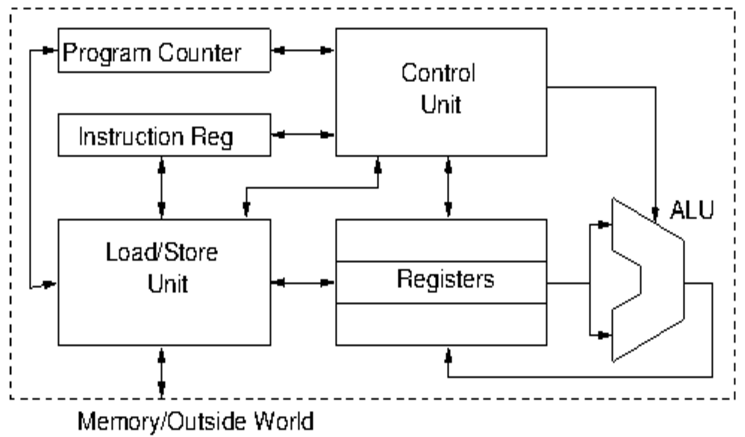
\includegraphics[width=0.6\textwidth]{von_neumann}
		\caption{The von Neumann Architecture}
		\label{fig:von neumann}
	\end{figure}
	
	Many modern computers are built on the (or use slightly modified) von Neumann\index{von Neumann architecture} architectures and can be considered it's heart. 
	
	\par	
	We consider the main memory\index{main memory} as being logically - but not necessarily physically - separate from the CPU. The main memory holds all of the instructions and data that make up a program(s). As stated earlier, instructions and data are stored in distinct locations within the main memory so that they are easily distinguished. Within main memory, instructions are stored sequentially so that you can determine the flow of the program implicitly from their order. Lastly, main memory is also a volatile\index{volatile} storage method, meaning that all data is lost once the power is cut.
	
	\par 
	The \textbf{Load/Store unit}\index{load/store unit} is used as the interface between the CPU and the outside world. It issues and receives requests to transfer instructions and data between the CPU and the memory via the bus.
	
	\par
	The \textbf{registers}\index{registers} are small amounts of local, fast access storage the hold data that is currently in use. Data is passed to the registers by the load/store unit. Each register can hold one 'word' of data. The main registers are used purely to hold data - instructions are dealt with separately.
	
	\par 
	The \textbf{instruction register}\index{instruction register} hold the current instruction that is being executed so that it can be used by the control unit\index{control unit} to configure the ALU\index{ALU}. Only one instruction is active at any one time, unless the design features special techniques for performance improvements that rely on multiple instructions being executed simultaneously.
	
	\par 
	The \textbf{ALU (arithmetic and logic unit)}\index{ALU}\index{arithmetic and logic unit} is the 'engine' of the computer. It performs all the computations and comparisons. It also reads data from registers and writes the results of calculations back into the registers.
	
	\par 
	The \textbf{program counter}\index{program counter} is a special register that contains the memory location (address) of the next instruction which shall be executed - a bookmark in essence. In the normal execution of a program, the program counter is incremented after each instruction to point to the next memory location. Some instructions may change the value of the program counter in order to change the order of execution.
	
	\par 
	Additionally, we may want to add some other components just outside of the CPU which can be just as important. Due to the fact the main memory is remote from the CPU, access times can be slow. We may use an intermediate layer of memory known as \textbf{cache}\index{cache} that is smaller but much faster to access. This would be used to hold portions of programs that are likely to be used again shortly. We may also want to use stable, \textbf{long-term memories}\index{long-term memory} such as disks or DVDs. Typically these all will require the use of an \textbf{Input-Output (IO) controller}\index{IO controller} which handles peripheral devices such as disk drives, mice and keyboards. It may do this through an extension of the memory addressing protocol or via an interrupt based protocol. Memory, peripherals and the CPU all communicate with each other via the \textbf{bus}\index{bus} which carries data around and allows, for example, data to be transferred from disk into main memory. This bus consists of a set of physical wires plus a protocol (there are many available, such as PCI, ISA, IDE, SCSI) that is implemented by the \textbf{bus controller}\index{bus controller}. The bus controller determines which subsystems can communicate. It should be noted that only one piece of data can be on the bus at any time.
	
	\subsubsection{The Clock Cycle}
	The vast, vast majority of computer systems are \textit{synchronous} - meaning their activities are synchronised by an external clock signal in the form of a \textbf{square-wave electric pulse}. This speed is frequently quoted as a measure of CPU performance but to say it is analogous to performance would be slightly false. There are many other factors and different architectures cannot be compared on the basis of their clock rate alone. The time between two different pulses is related to the frequency of the CPU by $t = 1 / f$ and is called a cycle time.
	
	\par 
	For the most part computer systems must be synchronus as variability in manufacturing means that it's not possible to know exactly how long it will take for a particular operation to complete. The clock cycle is chosen to be slightly longer than the longest delay in the system which ensure the machine is in a well defined state when the next set of operations start which is triggered by the \textbf{rising edge} of the clock pulse.
	
	\subsubsection{Executing Programs}	
	Computer programs, in their most basic form, are just sequential series' of instructions. In von Neumann architecture, the execution of these instructions is governed by the \textbf{instruction execution cycle}\index{instruction execution cycle}. The instruction execution cycle is triggered by the clock cycle, but has several stages within it which are triggered by successive clock pulses. One complete instruction cycle usually takes several clock cycles to execute - exact numbers depend on the type of instruction and the details of the particular machine. Fetch data from memory for example may take several clock cycles to execute, and it may take several cycles before the data is safely loaded into a register. Others may complete in a single clock cycle such as the addition of the contents of two values stored in registers.
	
	\par 
	Most architectures follow the same basic set of stages in the \textbf{Fetch-Decode-Execute Cycle}\index{fetch-decode-execute cycle}. In can roughly be broken down into 8 steps in an idealised version:
	
	\textbf{Fetch:}
	\begin{enumerate}
		\item Inspect the program counter to find the address of the next instruction
		\item Load the next instruction from memory into the instruction register
		\item Update the program counter to point at the next instruction
	\end{enumerate}
	
	\textbf{Decode:}
	\begin{enumerate}
		\setcounter{enumi}{4}
		\item Determine the type of instruction fetched
		\item If the instruction requires data from memory, determine its address (usually embedded in the instruction
	\end{enumerate}
	
	\textbf{Execute:}
	\begin{enumerate}
		\item Fetch and required data from memory into one of the CPU registers
		\item Execute the instruction
		\item Return to step 1 for the next instruction
	\end{enumerate}
	
	Starting a program doesn't fit neatly into this simple model and before we enter the cycle we also need to take a few actions to make sure that things are ready. Firstly, we need to load the program from disk into main memory\index{main memory}. The instructions and data needed by the program will each occupy a block of memory, which is allocated by the operating system, and the memory address of the first instruction is called the \textbf{entry point}\index{entry point}. When first started, the entry point is loaded into the program counter which then becomes the starting point of the cycle.
	
	\par 
	\textbf{Fetch}. Once we have a valid instruction location in the program counter (PC), we can begin the cycle. An important note is that at this point in time all we have is the memory address - not the actual instruction - we still need to actual fetch it, hence the title. At the start of the next clock cycle, the CPU issues a request via the load/store unit to the memory by sending the memory address and a request to read from the memory via the bus. Later in time, the instruction will be received from memory by the load/store unit and then stored in the instruction register (IR). Depending on the relative speed of the clock cycle and the memory, it could take several cycles before the instruction is ready in the IR. Once the request  has been made, the value of the PC is changed to point to the next instruction - which usually just involves simply incrementing the PC. This may however be modified by some instructions such as \texttt{branch} or \texttt{jump}.
	
	\par 
	\textbf{Decode}. Now we have the instruction in the IR, we can begin to act upon it in the CPU. The type of instruction is determined by the control unit. This is necessary in order to determine if any further actions needs to be taken in order to execute this instruction.
	
	\par 
	\textbf{Execute}. After finding the type of instruction, any data needed is fetched from the memory. For a lot of CPUs, most instructions can only actually access registers and there are dedicated instructions for accessing main memory. Once the data is in the registers, it can be operated upon. As mentioned earlier, some instructions change the flow of the program and are therefore allowed to change the PC as necessary (when doing this it is often required for the previous value of the PC to be stored so that execution can resume once the branch has completed).
	
	\subsection{Harvard Architecture}
	In the von Neumann architecture, instructions and data are accessed via the same physical and logical pathway (the load/store unit) and there is not formal separation between data and instructions at this level. In this case, the two types of information are stored in the same physical memory but are separated by their locations within the memory. This separation is common practice in all computers as it allows for dynamic repartitioning of the memory according to the needs of the program. The problem is due to the fact that by having a shared interface, instructions and data cannot be accessed simultaneously. This is known as the \textbf{von Neumann bottleneck}\index{von Neumann bottleneck} and it restricts CPU performance to the rate at which is can be supplied with data.
	
	\par 
	A potential solution is to provide separate memories for small amounts of instructions and data that are likely to be used soon - separate instruction and data caches. It is also common to provide separate interfaces to instruction and data memory which is known as the \textbf{Harvard architecture}\index{harvard architecture}. In a pure implementation of the Harvard model, instructions and data are stored in physically separate memory but this is not flexible enough for general purpose computational devices that has a single unified memory space. The \textbf{modified Harvard architecture} has a single unified memory space (that is partitioned for instructions and data) but with separate buses for instructions and data. In most modern machines, this is the approach that is taken.
	
	\subsection{Case Studies}
	\subsubsection{MIPS}
	The MIPS processor is the canonical example of a modified Harvard architecture and is very similar to the von Neumann model shown earlier. It features an instruction register, a program counter, an ALU etc, but has separate pathways for accessing instructions and for accessing data. In the diagram they are shown as physically separate, but in reality they are part of a physically unified memory.
	
	\begin{figure}[h]
		\centering
		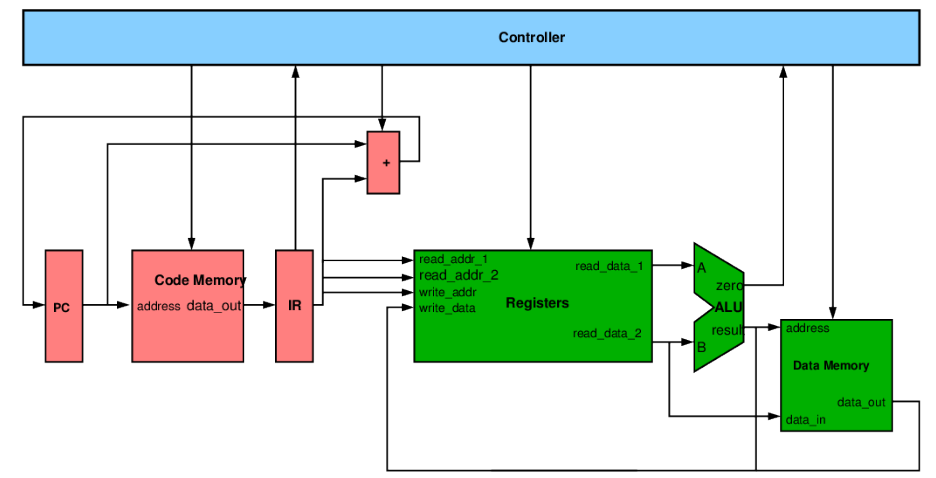
\includegraphics[width=\textwidth]{mips_architecture}
		\caption{The MIPS processor}
		\label{fig:mips processor}
	\end{figure}
	
	\subsubsection{Intel x86}
	Modern versions of x86 are much more complex when compared to the relatively simple MIPS Harvard based architecture. This is partly down to the fact that MIPS has around 60 simple instructions whereas the latest Intel Core machines have hundreds of instructions - many of which are not simple. The benefit of these additional instructions for the x86 architecture is a significant increase in performance and it can also make it easier for the programmer/compiler writer. This all comes at the cost of a much more complex design - MIPS R4000 contains 1.2 million transistors. A quad-core i7 processor on the other hand has 731 million transistors on a die that is not much larger than that in a MIPS machine. One of the main features of modern Core architecture is that it is highly superscalar and can execute multiple instructions simultaneously. Due to this, the CPU requires several ALUs, several instruction decoders, instruction queues and multiple levels of caching. If you can see through all the complexity, you can see that the Core 2 is essentially a modified Harvard architecture.
	
	\section{Instruction Sets and Assembly Language}
	
	\section{CPU Microarchitecture}
	
	\section{Digital Logic}
	
	\section{I/O and Peripherals}
	
	\section{Improving Performance}
	
	\newpage
	\listoffigures
	\printindex	
\end{document}